
\documentclass[aspectratio=169,11pt]{beamer}
\usetheme{Madrid}
\usecolortheme{seahorse}
\usefonttheme{professionalfonts}
\usepackage{amsmath,amssymb,bm,booktabs,array,graphicx,hyperref,multicol}
\usepackage{xcolor,xeCJK,fontspec}
\graphicspath{{../outputs/paper/figures/}{../outputs/}}
\setmainfont{texgyreheros-regular.otf}[BoldFont=texgyreheros-bold.otf,ItalicFont=texgyreheros-italic.otf]
\setsansfont{texgyreheros-regular.otf}[BoldFont=texgyreheros-bold.otf,ItalicFont=texgyreheros-italic.otf]
\setmonofont{lmmono10-regular.otf}[BoldFont=lmmonolt10-bold.otf]
\setCJKmainfont{FandolHei-Regular.otf}
\setCJKsansfont{FandolHei-Regular.otf}
\setCJKmonofont{FandolFang-Regular.otf}
\definecolor{myblue}{RGB}{36,88,135}
\definecolor{mygreen}{RGB}{40,120,80}
\definecolor{myorange}{RGB}{180,100,30}
\definecolor{mygray}{RGB}{90,90,90}
\setbeamercolor{title}{fg=myblue}
\setbeamercolor{frametitle}{fg=myblue}
\setbeamercolor{structure}{fg=myblue}
\setbeamercolor{block title}{bg=myblue,fg=white}
\setbeamercolor{block body}{bg=blue!5,fg=black}
\setbeamercolor{alertblock title}{bg=myorange,fg=white}
\setbeamercolor{alertblock body}{bg=orange!8,fg=black}
\setbeamercolor{exampleblock title}{bg=mygreen,fg=white}
\setbeamercolor{exampleblock body}{bg=green!6,fg=black}
\setbeamertemplate{navigation symbols}{}
\setbeamertemplate{footline}[frame number]
\newcommand{\R}{\mathbb{R}}
\title[Week 8]{Week 8: 论文组织、结果复现与项目展示}
\subtitle{From three-phase N-1 experiments to a reproducible mini-paper}
\author{ECE Course: Physics-informed AI for Microgrid Security Prediction}
\date{}
\begin{document}

\begin{frame}\titlepage\end{frame}

\begin{frame}{本周学习目标}
\begin{enumerate}
  \item 把 Weeks 3--7 的结果组织成一套可复现科研包。
  \item 将三相 N-1 安全筛查流程转写为 mini-paper 的问题定义、方法和实验。
  \item 为每个论文 claim 配置可检查的 evidence。
  \item 生成 paper-ready tables、figures、LaTeX skeleton 和 presentation outline。
  \item 用 validation summary、hash manifest、no-leakage audit 证明结果链路可信。
\end{enumerate}
\end{frame}

\begin{frame}{八周课程闭环}
\small
\begin{block}{从教学到论文}
\texttt{Week 1 pandapower} $\rightarrow$ \texttt{Week 2 three-phase PF} $\rightarrow$ \texttt{Week 3 scenarios} $\rightarrow$ \texttt{Week 4 N-1 labels} $\rightarrow$ \texttt{Week 5 ML} $\rightarrow$ \texttt{Week 6 PI-MLP} $\rightarrow$ \texttt{Week 7 GNN} $\rightarrow$ \texttt{Week 8 paper package}
\end{block}
\begin{itemize}
  \item Week 8 不再增加新模型，而是做科研闭环。
  \item 目标是让学生知道：实验结果必须被整理为可验证、可复现、可写作的证据链。
  \item 最终输出包括 mini-paper、presentation outline、artifact manifest 和 validation summary。
\end{itemize}
\end{frame}

\begin{frame}{最终科研故事线}
\begin{block}{一句话}
三相不平衡微电网的 N-1 安全评估需要大量 \texttt{runpp\_3ph()} 扫描；我们用 pandapower 生成可复现 ground truth，再用 ML / PI-MLP / GNN 学习 contingency risk，以 high-recall screening 减少后续三相潮流调用。
\end{block}
\begin{alertblock}{部署定位}
AI 是 pre-screening module。它用于排序和筛查高风险 contingency，不直接替代潮流计算、保护配置或运行员判断。
\end{alertblock}
\end{frame}

\begin{frame}{论文问题定义}
给定 operating scenario $x_t$ 和 contingency $c$，学习
\[
(x_t,c) \mapsto \hat p_{t,c} = \Pr(y_{t,c}=1), \qquad \hat s_{t,c}
\]
\begin{itemize}
  \item $x_t$：base-case 三相微电网状态，包括负荷、PV、BESS、base-case voltage / loading / VUF。
  \item $c$：line outage、PV trip、BESS trip 或 PCC outage。
  \item $y_{t,c}$：是否出现 voltage / loading / VUF / service-loss / convergence violation。
  \item $s_{t,c}$：violation severity 或 component margin 的合成指标。
\end{itemize}
\end{frame}

\begin{frame}{为什么目标不是 Accuracy}
\begin{columns}
\begin{column}{0.54\textwidth}
\begin{itemize}
  \item 安全筛查中最危险错误是 false negative。
  \item 高 accuracy 可能来自“多数类”而不是安全可靠性。
  \item threshold 只能用 validation set 选择。
  \item test set 只用于最终报告。
\end{itemize}
\end{column}
\begin{column}{0.44\textwidth}
\[
\mathrm{Recall}=\frac{TP}{TP+FN}
\]
\[
\mathrm{FNR}=\frac{FN}{TP+FN}
\]
\[
\mathrm{PFsaved}=\frac{TN+FN}{N}
\]
\end{column}
\end{columns}
\begin{block}{论文表述}
我们优先报告 recall、FNR、missed violations 和 saved PF calls，而不是单独强调 accuracy。
\end{block}
\end{frame}

\begin{frame}{Week 8 最终交付物}
\begin{enumerate}
  \item \textbf{Mini-paper skeleton}：IEEEtran 风格 LaTeX 初稿。
  \item \textbf{Paper-ready tables}：dataset、model comparison、group CV、ablation。
  \item \textbf{Paper figures}：label distribution、PR curves、screening tradeoff、top-k recall。
  \item \textbf{Final presentation outline}：10--15 页答辩结构。
  \item \textbf{Reproducibility package}：artifact hash manifest、validation checks、claim-evidence table。
\end{enumerate}
\end{frame}

\begin{frame}{Mini-paper 推荐结构}
\small
\begin{enumerate}
  \item Introduction
  \item Three-phase microgrid security formulation
  \item Dataset generation with pandapower
  \item ML / PI-MLP / GNN screening methods
  \item Experimental setup
  \item Results and ablation studies
  \item Discussion and limitations
  \item Conclusion
\end{enumerate}
\begin{block}{写作重点}
不要把 Notebook 变成论文。论文需要问题、方法、证据、限制和结论之间的逻辑链。
\end{block}
\end{frame}

\begin{frame}{Introduction 怎么写}
\begin{enumerate}
  \item \textbf{背景}：microgrid / LV feeder 中单相负荷、PV、EV、BESS 导致三相不平衡。
  \item \textbf{痛点}：大量 scenario 和 contingency 使三相 N-1 全扫描成本高。
  \item \textbf{机会}：AI 可以作为高召回预筛查器。
  \item \textbf{风险}：AI 可能漏报危险 contingency，因此需要 validation discipline。
\end{enumerate}
\begin{exampleblock}{贡献写法}
``We propose a reproducible phase-aware N-1 labeling and screening workflow for unbalanced microgrids.''
\end{exampleblock}
\end{frame}

\begin{frame}{Problem Formulation 怎么写}
\small
需要清楚定义：
\begin{itemize}
  \item scenario set $\mathcal{T}$ 和 contingency catalog $\mathcal{C}$；
  \item post-contingency 三相结果 $V_{i,\phi}^c$、$I_{\ell,\phi}^c$、VUF；
  \item voltage low / high、line loading、VUF、service-loss、non-convergence 标签；
  \item binary label $y_{t,c}$ 与 severity score $s_{t,c}$；
  \item high-recall screening objective。
\end{itemize}
\[
y_{t,c} = \mathbf{1}\left(\bigvee_k m_{t,c}^k >0\right),\qquad s_{t,c} = \max_k m_{t,c}^k
\]
\end{frame}

\begin{frame}{Dataset Generation Section 怎么写}
\begin{itemize}
  \item Week 3：构造 microgrid-like feeder，定义 scenario table。
  \item Week 4：组合 scenario 和 contingency，运行三相 N-1 labeling。
  \item 每一行样本对应 $(x_t,c)$。
  \item 每个标签都可以追溯到 post-contingency proof：VUF、line loading、service-loss、convergence status。
\end{itemize}
\begin{block}{关键原则}
Dataset section 不只写“生成了数据”，还要写清楚标签如何定义、如何验证、如何避免泄漏。
\end{block}
\end{frame}

\begin{frame}{Method Section: 三层模型}
\begin{enumerate}
  \item \textbf{Engineering rule / traditional ML}：建立可信 baseline。
  \item \textbf{PI-MLP}：多任务输出 probability、severity、component margins。
  \item \textbf{Phase-aware GNN}：把 bus、line、contingency mask 和三相 channels 作为图输入。
\end{enumerate}
\begin{alertblock}{写作建议}
不要只展示最终模型。逐层 baseline 更容易说明“改进来自哪里”。
\end{alertblock}
\end{frame}

\begin{frame}{PI-MLP Loss 写法}
\[
\mathcal{L}=
\mathcal{L}_{BCE}
+\lambda_s\mathcal{L}_{sev}
+\lambda_m\mathcal{L}_{margin}
+\lambda_c\mathcal{L}_{consistency}
+\lambda_r\mathcal{L}_{rank}
\]
\begin{itemize}
  \item $\mathcal{L}_{BCE}$：violation classification。
  \item $\mathcal{L}_{sev}$：severity regression。
  \item $\mathcal{L}_{margin}$：voltage / loading / service-loss margin targets。
  \item $\mathcal{L}_{rank}$：让更严重 contingency 的风险分数更高。
\end{itemize}
\end{frame}

\begin{frame}{GNN Section 怎么写}
\begin{itemize}
  \item Node features：bus-level A/B/C phase-channel features。
  \item Edge features：line parameters、edge availability、outage mask。
  \item Global features：scenario metadata 和 contingency type。
  \item Output：graph-level risk score $\hat p_{t,c}$。
  \item Validation：edge-order / node-order permutation invariance proof。
\end{itemize}
\begin{block}{诚实表达}
小数据下 GNN 不一定优于 MLP。它的价值在于拓扑建模和后续扩展空间。
\end{block}
\end{frame}

\begin{frame}{Dataset Statistics}
\centering
\begin{tabular}{lr}
\toprule
Quantity & Value \\
\midrule
Scenarios & 7 \\
Contingencies & 11 \\
Scenario-contingency samples & 77 \\
Safe samples & 30 \\
Unsafe samples & 47 \\
PF-solved rows & 35 \\
Service-loss skipped rows & 35 \\
No-slack skipped rows & 7 \\
\bottomrule
\end{tabular}
\end{frame}

\begin{frame}{Violation Type Summary}
\centering
\scriptsize
\begin{tabular}{lr}
\toprule
Violation type & Count \\
\midrule
voltage\_low\_violation & 5 \\
voltage\_high\_violation & 0 \\
loading\_violation & 5 \\
vuf\_violation & 0 \\
non\_convergence\_violation & 7 \\
service\_loss\_violation & 42 \\
critical\_service\_loss\_violation & 28 \\
\bottomrule
\end{tabular}
\begin{block}{解读}
教学数据集中 service-loss 是主要风险类型；voltage 和 loading violation 数量较少，适合说明类别不平衡和高召回筛查的重要性。
\end{block}
\end{frame}

\begin{frame}{Figure: Label Distribution by Contingency Type}
\centering
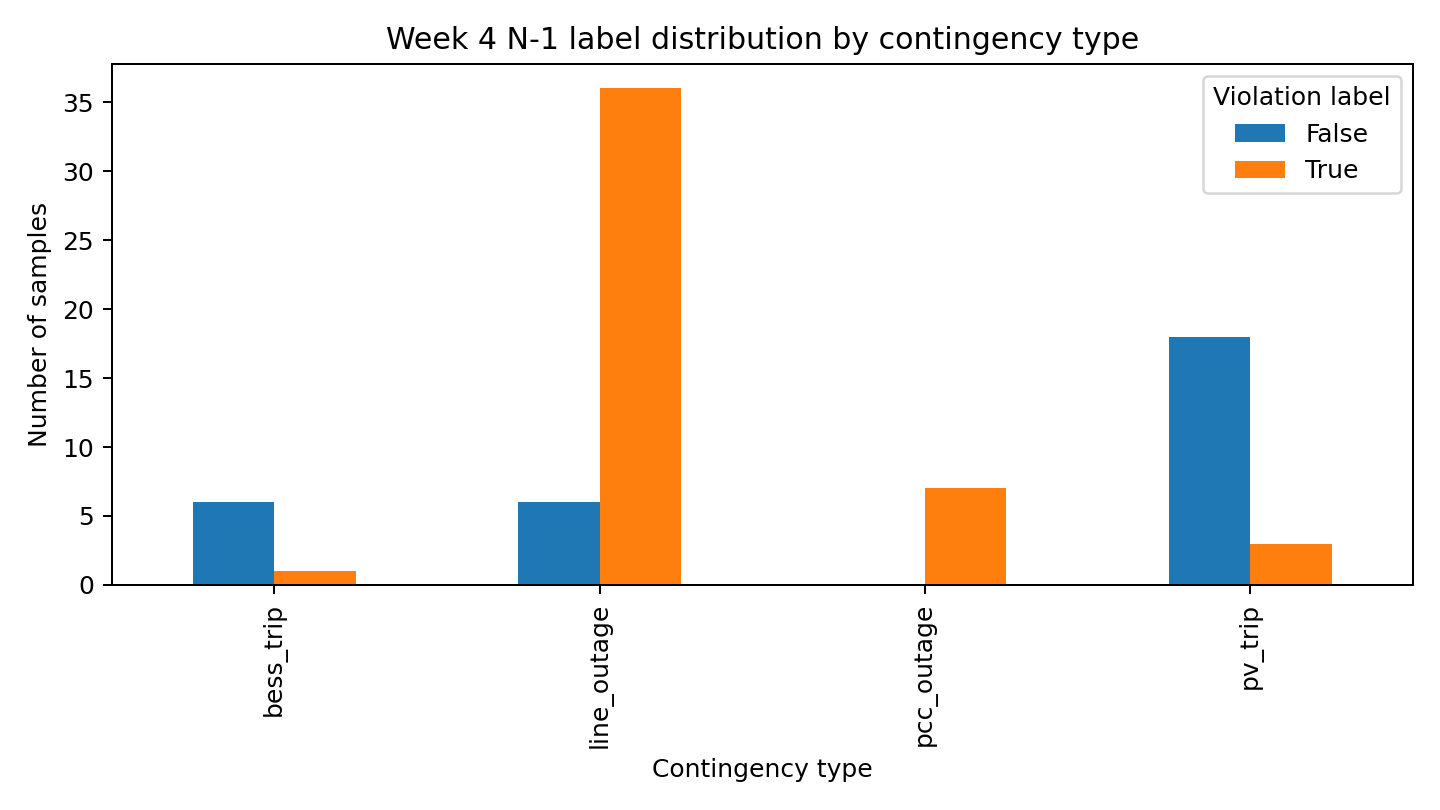
\includegraphics[width=0.82\textwidth]{fig1_week4_label_distribution_by_type.png}
\end{frame}

\begin{frame}{Figure: Severity Distribution}
\centering
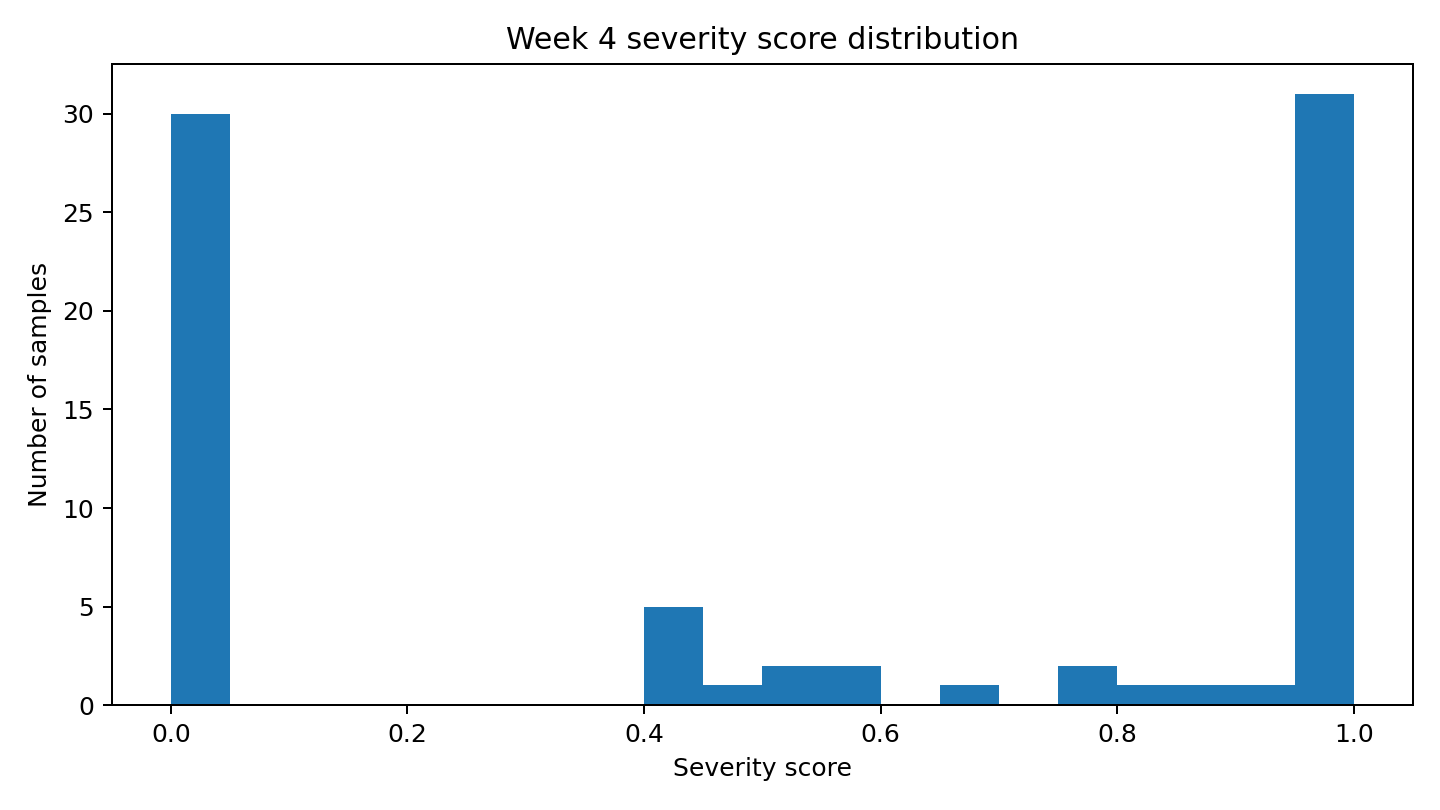
\includegraphics[width=0.82\textwidth]{fig2_week4_severity_distribution.png}
\end{frame}

\begin{frame}{Holdout Model Comparison}
\centering
\scriptsize
\resizebox{\textwidth}{!}{%
\begin{tabular}{llrrrrr}
\toprule
Stage & Model & Recall & Precision & FNR & PF saved & Missed \\
\midrule
W5 ML baseline & GradientBoosting & 1.000 & 1.000 & 0.000 & 0.400 & 0 \\
W6 PI-MLP & PI-MLP full & 1.000 & 1.000 & 0.000 & 0.400 & 0 \\
W7 GNN & FlattenedMLP & 1.000 & 1.000 & 0.000 & 0.400 & 0 \\
W5 ML baseline & EngineeringRule & 1.000 & 0.857 & 0.000 & 0.300 & 0 \\
W6 PI-MLP & BaselineMLP & 1.000 & 0.857 & 0.000 & 0.300 & 0 \\
W5 ML baseline & AllUnsafe & 1.000 & 0.600 & 0.000 & 0.000 & 0 \\
W5 ML baseline & MLP & 1.000 & 0.600 & 0.000 & 0.000 & 0 \\
W5 ML baseline & LogisticRegression & 0.833 & 1.000 & 0.167 & 0.500 & 2 \\
\bottomrule
\end{tabular}
}
\end{frame}

\begin{frame}{如何解读 Holdout 结果}
\begin{itemize}
  \item 多个模型达到 zero missed violations，但 saved PF calls 不同。
  \item GradientBoosting、PI-MLP full 和 FlattenedMLP 在 holdout 中都达到 recall=1.0、missed=0、PF saved=0.4。
  \item PhaseAwareGNN 在小数据上表现较弱，这是重要 limitation，而不是需要隐藏的结果。
\end{itemize}
\begin{alertblock}{写作原则}
论文里必须区分“教学样例结果”和“可部署泛化结论”。
\end{alertblock}
\end{frame}

\begin{frame}{Figure: Precision-Recall Curves}
\centering
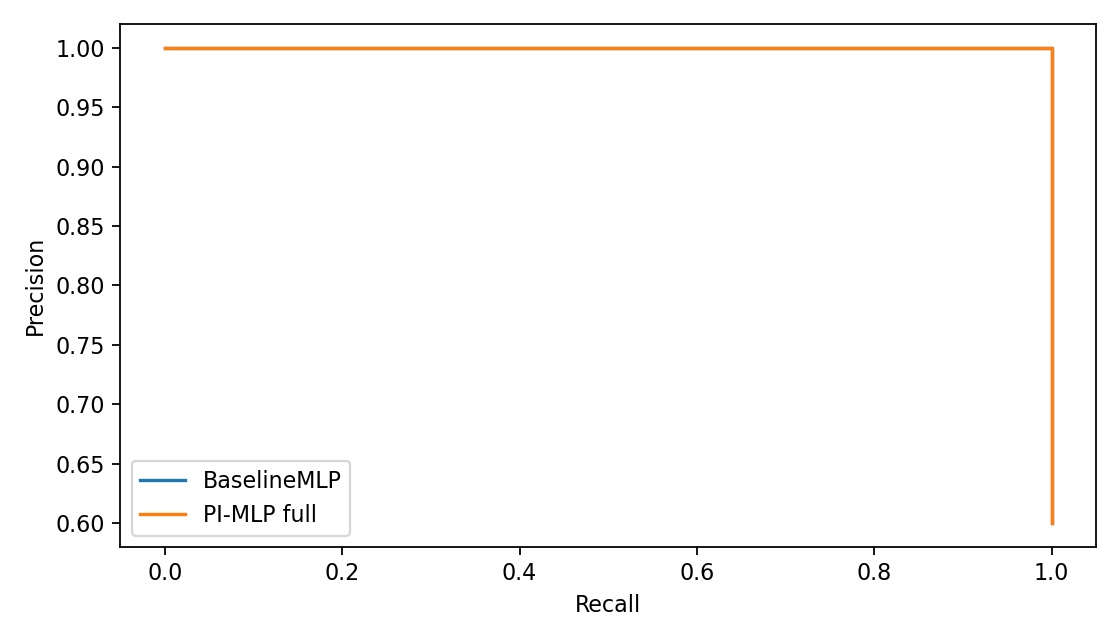
\includegraphics[width=0.82\textwidth]{fig3_week6_precision_recall_curves.png}
\end{frame}

\begin{frame}{Figure: Saved PF Calls vs Missed Violations}
\centering
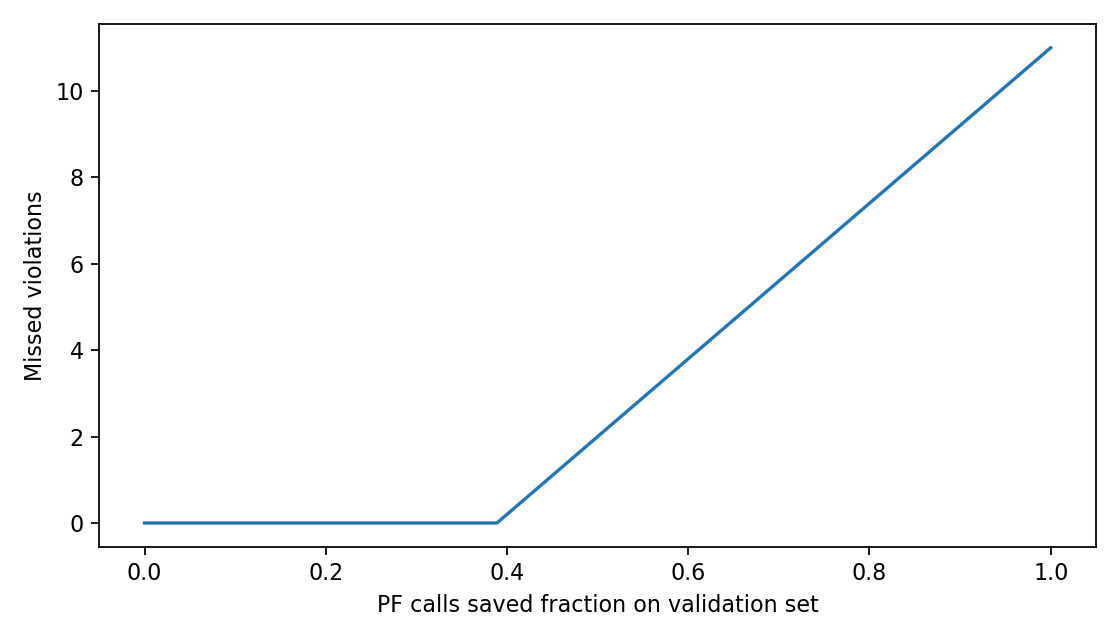
\includegraphics[width=0.82\textwidth]{fig4_week6_saved_calls_vs_missed_violations.png}
\end{frame}

\begin{frame}{OOD-style Group CV}
\centering
\scriptsize
\resizebox{\textwidth}{!}{%
\begin{tabular}{lrrrrr}
\toprule
Model & Split & Folds & Mean recall & Mean FNR & Mean PF saved \\
\midrule
EngineeringRule & scenario-group & 3 & 1.000 & 0.000 & 0.323 \\
RandomForest & scenario-group & 3 & 0.899 & 0.101 & 0.475 \\
EngineeringRule & contingency-group & 3 & 1.000 & 0.000 & 0.310 \\
RandomForest & contingency-group & 3 & 0.400 & 0.600 & 0.690 \\
PI-MLP full & contingency-group & 3 & 0.760 & 0.240 & 0.413 \\
PI-MLP full & scenario-group & 3 & 0.928 & 0.072 & 0.207 \\
PhaseAwareGNN & contingency-group & 11 & 0.896 & 0.104 & 0.247 \\
PhaseAwareGNN & scenario-group & 7 & 0.690 & 0.310 & 0.468 \\
\bottomrule
\end{tabular}
}
\begin{block}{为什么要做 group CV}
Random split 可能让相同 scenario 或 contingency 同时出现在训练和测试中；group split 用于测试更难的泛化。
\end{block}
\end{frame}

\begin{frame}{Group Split Proof}
对每个 fold 都必须证明：
\[
\mathcal{G}_{train} \cap \mathcal{G}_{test} = \emptyset
\]
\begin{itemize}
  \item Scenario-group CV：测试未见过的 operating scenario。
  \item Contingency-group CV：测试未见过的 contingency。
  \item 这是比 random holdout 更严格的证据。
\end{itemize}
\begin{exampleblock}{Notebook 08 的做法}
读取 Week 5--7 的 CV 结果，并检查 CV metrics 在 $[0,1]$ 内且文件非空。
\end{exampleblock}
\end{frame}

\begin{frame}{Top-k Contingency Screening}
\centering
\scriptsize
\begin{tabular}{rrrrr}
\toprule
$k$ & PF call fraction & Mean recall@k & Min recall@k & Severe hit@k \\
\midrule
1 & 0.091 & 0.156 & 0.091 & 1.000 \\
3 & 0.273 & 0.468 & 0.273 & 1.000 \\
5 & 0.455 & 0.636 & 0.455 & 1.000 \\
7 & 0.636 & 0.948 & 0.636 & 1.000 \\
11 & 1.000 & 1.000 & 1.000 & 1.000 \\
\bottomrule
\end{tabular}
\begin{block}{部署解释}
如果运行员只想精算前 $k$ 个 contingency，top-k recall 衡量危险样本是否被排在高优先级列表中。
\end{block}
\end{frame}

\begin{frame}{Figure: Top-k Violation Recall}
\centering
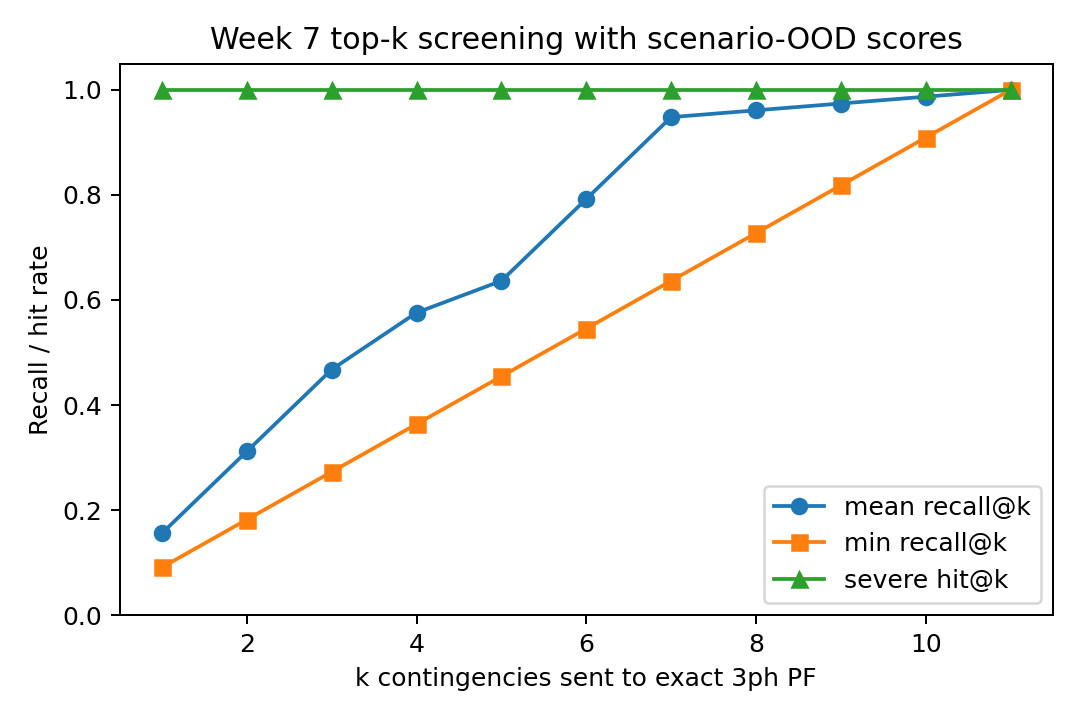
\includegraphics[height=0.76\textheight,keepaspectratio]{fig5_week7_topk_violation_recall.png}
\end{frame}

\begin{frame}{Figure: Group CV Recall}
\centering
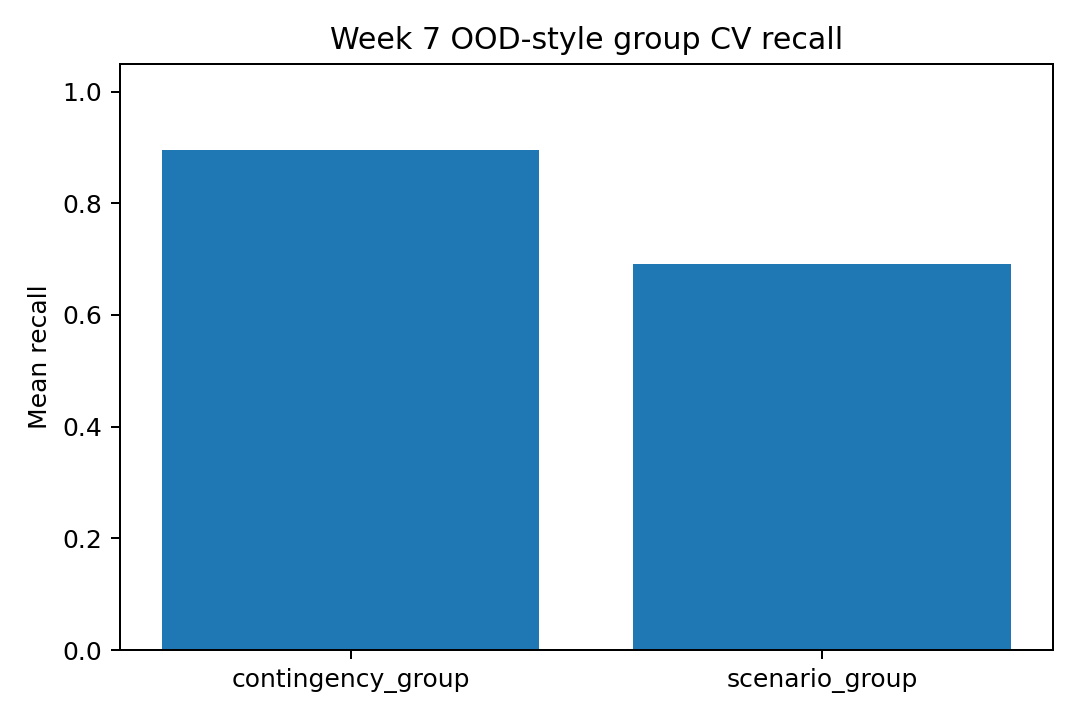
\includegraphics[height=0.76\textheight,keepaspectratio]{fig6_week7_group_cv_recall.png}
\end{frame}

\begin{frame}{Figure: True vs Predicted Severity}
\centering
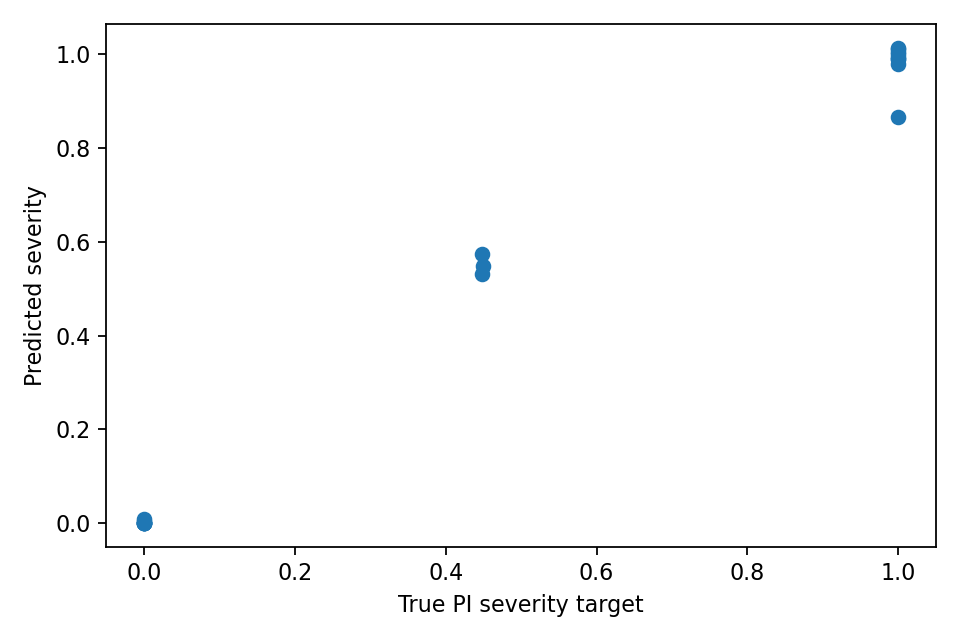
\includegraphics[height=0.76\textheight,keepaspectratio]{fig7_week6_true_vs_predicted_severity.png}
\end{frame}

\begin{frame}{Validation Suite Summary}
\centering
\begin{tabular}{lrrc}
\toprule
Week & Checks & Passed & All passed \\
\midrule
Week 3 & 12 & 12 & True \\
Week 4 & 13 & 13 & True \\
Week 5 & 12 & 12 & True \\
Week 6 & 16 & 16 & True \\
Week 7 & 44 & 44 & True \\
\bottomrule
\end{tabular}
\begin{block}{核心信息}
Week 8 的论文表格不是孤立结果，而是建立在 Weeks 3--7 的 validation suite 之上。
\end{block}
\end{frame}

\begin{frame}{Dataset Lineage Proof}
\[
N_{samples} = N_{scenarios} \times N_{contingencies}
\]
\vspace{-0.8cm}
\[
77 = 7 \times 11
\]
\begin{itemize}
  \item 每个 $(scenario\_id, contingency\_id)$ 只出现一次。
  \item Week 4 N-1 dataset 与 AI-ready dataset 行数一致。
  \item safe / unsafe 统计与 violation label 一致。
\end{itemize}
\end{frame}

\begin{frame}{No-leakage Proof}
\begin{columns}
\begin{column}{0.50\textwidth}
\textbf{禁止作为输入}
\begin{itemize}
  \item post-contingency voltage / loading / VUF
  \item violation flags
  \item severity score
  \item convergence / service-loss label
\end{itemize}
\end{column}
\begin{column}{0.50\textwidth}
\textbf{允许作为输入}
\begin{itemize}
  \item base-case summary
  \item scenario settings
  \item device metadata
  \item contingency identity and location
\end{itemize}
\end{column}
\end{columns}
\begin{block}{Notebook 08 输出}
\texttt{week8\_feature\_leakage\_audit.csv} 复查 Week 5 和 Week 7 特征列表。
\end{block}
\end{frame}

\begin{frame}{Metric Consistency Proof}
Notebook 必须手算 confusion matrix，再复核指标：
\[
TP,FP,TN,FN
\]
\[
\mathrm{Recall}=\frac{TP}{TP+FN},\qquad
\mathrm{Precision}=\frac{TP}{TP+FP}
\]
\[
\mathrm{PFsaved}=\frac{TN+FN}{N},\qquad
\mathrm{Missed}=FN
\]
\begin{alertblock}{不要只依赖库函数}
安全筛查指标要让学生看懂每一个 missed violation 是如何进入结果表的。
\end{alertblock}
\end{frame}

\begin{frame}{Artifact Manifest and Hash Proof}
\begin{itemize}
  \item \texttt{week8\_artifact\_manifest.csv} 记录核心输入输出文件。
  \item 每个 artifact 包含 path、type、size 和 SHA256 hash。
  \item 这可以帮助学生检查文件是否被替换、截断或错误复制。
\end{itemize}
\begin{block}{论文包原则}
没有进入 manifest 的结果，不应该出现在最终论文 claim 中。
\end{block}
\end{frame}

\begin{frame}{Claim-Evidence Table}
\centering
\scriptsize
\resizebox{\textwidth}{!}{%
\begin{tabular}{llc}
\toprule
ID & Claim & Status \\
\midrule
C1 & The workflow creates a complete three-phase N-1 dataset from scenario an... & supported \\
C2 & The binary violation label is consistent with voltage, loading, VUF, ser... & supported \\
C3 & The best zero-missed-violation holdout model is GradientBoosting with PF... & supported \\
C4 & Group-based CV provides a stricter test than random holdout because scen... & supported \\
C5 & Top-k screening provides an operator-oriented way to reduce the continge... & supported \\
L1 & The current benchmark is a small teaching feeder, so results should not ... & limitation \\
\bottomrule
\end{tabular}
}
\begin{block}{写作习惯}
每一条 claim 都要能指向表格、图、validation proof 或明确 limitation。
\end{block}
\end{frame}

\begin{frame}{Reproducibility Checklist}
\centering
\scriptsize
\resizebox{\textwidth}{!}{%
\begin{tabular}{llc}
\toprule
Item & Description & Passed \\
\midrule
data\_lineage & Scenario count × contingency count equals N-1 dataset rows. & True \\
label\_consistency & Final violation label equals OR of all component violation flags. & True \\
validation\_summaries & Week 3--7 validation summaries all pass. & True \\
no\_leakage & Feature lists do not include post-contingency labels or metrics. & True \\
threshold\_protocol & Threshold is selected on validation set, not test set. & True \\
group\_cv & Scenario-group and contingency-group CV results are included. & True \\
topk & Top-k screening table is finite and monotonic. & True \\
paper\_tables & LaTeX tables are generated under paper/tables. & True \\
\bottomrule
\end{tabular}
}
\end{frame}

\begin{frame}{Mini-paper Skeleton}
Notebook 08 自动生成：
\begin{itemize}
  \item \texttt{paper/main.tex}
  \item \texttt{paper/tables/table1\_dataset\_statistics.tex}
  \item \texttt{paper/tables/table2\_model\_comparison.tex}
  \item \texttt{paper/tables/table3\_group\_cv.tex}
  \item \texttt{paper/tables/table4\_loss\_ablation.tex}
\end{itemize}
\begin{exampleblock}{学生任务}
补充 Introduction、Related Work、Method 细节和 Discussion，而不是重新造表。
\end{exampleblock}
\end{frame}

\begin{frame}{Final Presentation 推荐结构}
\small
\begin{enumerate}
  \item Problem and motivation
  \item Three-phase microgrid setting
  \item N-1 label generation
  \item AI screening formulation
  \item Baseline and PI-MLP
  \item Phase-aware GNN
  \item Results and tradeoff
  \item Validation suite
  \item Limitations
  \item Future work
\end{enumerate}
\end{frame}

\begin{frame}{Limitation 怎么写}
建议诚实写：
\begin{itemize}
  \item 当前数据集是 teaching feeder，小样本结果不能直接声称可部署泛化。
  \item Islanded mode 尚未完整建模，PCC outage 在 MVP 中被处理为 no-slack skip。
  \item PI loss 是 limit-aware / consistency-aware，不是严格 AC feasibility guarantee。
  \item GNN 在小数据下未必优于 MLP，需要更多 feeder 和 stochastic scenarios。
  \item 尚缺少真实 microgrid 数据验证。
\end{itemize}
\end{frame}

\begin{frame}{期刊扩展路线}
\begin{itemize}
  \item 增加 feeder 数量和 stochastic operating scenarios。
  \item 从 bus-level phase-channel GNN 扩展到 phase-level GNN。
  \item 加入 conformal prediction / selective classification，控制漏报风险。
  \item 引入 BESS SOC time series 和 inverter reactive power control。
  \item 建模 islanded microgrid 和 grid-forming inverter。
  \item 使用真实 microgrid 或 utility feeder 数据做外部验证。
\end{itemize}
\end{frame}

\begin{frame}{Notebook 08 输出}
\begin{itemize}
  \item \texttt{week8\_dataset\_lineage\_summary.csv}
  \item \texttt{week8\_model\_comparison\_table.csv}
  \item \texttt{week8\_group\_cv\_synthesis.csv}
  \item \texttt{week8\_claim\_evidence\_table.csv}
  \item \texttt{week8\_reproducibility\_checklist.csv}
  \item \texttt{paper/main.tex}
  \item \texttt{presentation/final\_presentation\_outline.md}
\end{itemize}
\begin{block}{Validation}
Week 8 主 validation checks: 22/22 passed；supplemental checks: 4/4 passed。
\end{block}
\end{frame}

\begin{frame}{课堂练习}
\begin{enumerate}
  \item 修改 mini-paper Introduction 的第一段，让问题动机更强。
  \item 从 paper figures 中选择最有说服力的 3 张图。
  \item 写 5 条 claims，并用 claim-evidence table 绑定证据。
  \item 根据 validation audit 找出一个诚实 limitation。
  \item 准备一个 5 分钟项目汇报。
\end{enumerate}
\end{frame}

\begin{frame}{Takeaways}
\begin{enumerate}
  \item 三相 N-1 安全筛查可以被系统化地数据化。
  \item High-recall screening 比单纯 accuracy 更符合安全应用。
  \item Physics-informed targets 和 graph representation 是研究方向，不是自动性能保证。
  \item 每一个实验结论都要有 artifact、proof 和 validation 支撑。
  \item 最终科研成果来自“模型 + 数据 + 证据链 + 诚实限制”。
\end{enumerate}
\end{frame}

\end{document}
